% ----------------------------------------------------------------- %
%             The Speech Signal Processing Toolkit (SPTK)           %
%             developed by SPTK Working Group                       %
%             http://sp-tk.sourceforge.net/                         %
% ----------------------------------------------------------------- %
%                                                                   %
%  Copyright (c) 1984-2007  Tokyo Institute of Technology           %
%                           Interdisciplinary Graduate School of    %
%                           Science and Engineering                 %
%                                                                   %
%                1996-2016  Nagoya Institute of Technology          %
%                           Department of Computer Science          %
%                                                                   %
% All rights reserved.                                              %
%                                                                   %
% Redistribution and use in source and binary forms, with or        %
% without modification, are permitted provided that the following   %
% conditions are met:                                               %
%                                                                   %
% - Redistributions of source code must retain the above copyright  %
%   notice, this list of conditions and the following disclaimer.   %
% - Redistributions in binary form must reproduce the above         %
%   copyright notice, this list of conditions and the following     %
%   disclaimer in the documentation and/or other materials provided %
%   with the distribution.                                          %
% - Neither the name of the SPTK working group nor the names of its %
%   contributors may be used to endorse or promote products derived %
%   from this software without specific prior written permission.   %
%                                                                   %
% THIS SOFTWARE IS PROVIDED BY THE COPYRIGHT HOLDERS AND            %
% CONTRIBUTORS "AS IS" AND ANY EXPRESS OR IMPLIED WARRANTIES,       %
% INCLUDING, BUT NOT LIMITED TO, THE IMPLIED WARRANTIES OF          %
% MERCHANTABILITY AND FITNESS FOR A PARTICULAR PURPOSE ARE          %
% DISCLAIMED. IN NO EVENT SHALL THE COPYRIGHT OWNER OR CONTRIBUTORS %
% BE LIABLE FOR ANY DIRECT, INDIRECT, INCIDENTAL, SPECIAL,          %
% EXEMPLARY, OR CONSEQUENTIAL DAMAGES (INCLUDING, BUT NOT LIMITED   %
% TO, PROCUREMENT OF SUBSTITUTE GOODS OR SERVICES; LOSS OF USE,     %
% DATA, OR PROFITS; OR BUSINESS INTERRUPTION) HOWEVER CAUSED AND ON %
% ANY THEORY OF LIABILITY, WHETHER IN CONTRACT, STRICT LIABILITY,   %
% OR TORT (INCLUDING NEGLIGENCE OR OTHERWISE) ARISING IN ANY WAY    %
% OUT OF THE USE OF THIS SOFTWARE, EVEN IF ADVISED OF THE           %
% POSSIBILITY OF SUCH DAMAGE.                                       %
% ----------------------------------------------------------------- %
\hypertarget{gmm}{}
\name[ref:GMMMAP-IEEE]{gmm}{GMM parameter estimation}{model training}

\begin{synopsis}
\item [gmm] [ --l $L$ ] [ --m $M$ ] [ --s $S$ ] [ --a $A$ ] [ --b $B$ ]
        [ --e $E$ ] [ --v $V$ ] [ --w $W$ ] [ --f ]
\item [\ ~~~~]  [ --M $W_{MAP}$ ][ --F $gmmfile$ ] [ --B $B1,B2,...$ ] [ --c1 ] [ --c2 ] [ {\em infile} ]
\end{synopsis}

\newfont{\bggg}{cmr10 scaled\magstep3}
\newcommand{\bigzerol}{\smash{\hbox{\bggg 0}}}
\newcommand{\bigzerou}{\smash{\lower1.3ex\hbox{\bggg 0}}}
\newcommand{\argmax}{\mathop{\rm argmax}\limits}

\begin{qsection}{DESCRIPTION}
{\em gmm} uses the expectation maximization (EM) algorithm to estimate
Gaussian mixture model (GMM) parameters with diagonal covariance
matrices, from a sequence of vectors in the {\em infile} (or standard
input), sending the result to standard output.

The input sequence $\bX$ consists of $T$ float vectors $\bx$, each of
size $L$:
\begin{align}
 &\bX=\left[\bx(0), \bx(1), \dots, \bx(T-1)\right]\notag,\\
 &\bx(t)=\left[x_t(0), x_t(1), \ldots, x_t(L-1)\right].\notag
\end{align}
The result is GMM parameters $\lambda$ consisting of $M$ mixture weights
$\bw$ and $M$ Gaussians with mean vector $\bmu$ and variance vector
$\bv$, each of length $L$:
\begin{align}
 \lambda =
 \left[\bw,\right.&\left.\bmu(0),\bv(0), \bmu(1), \bv(1),
 \ldots, \bmu(M-1), \bv(M-1)\right],\notag\\[2mm]
 \bw &=\left[ w(0), w(1), \ldots, w(M-1) \right],\notag\\
 \bmu(m) &=\left[\mu_m(0), \mu_m(1), \ldots, \mu_m(L-1)\right],\notag\\
 \bv(m) &=\left[\sigma_m^2(0), \sigma_m^2(1), \ldots,
 \sigma_m^2(L-1)\right],\notag
\end{align}
where
\begin{displaymath}
 \sum_{m=0}^{M-1}w(m)=1.
\end{displaymath}

The GMM parameter set $\lambda$ is initialized by an LBG algorithm and
the following EM steps are used iteratively to obtain the new parameter set
$\hat{\lambda}$:
\begin{align}
   \hat{w}(m) & = \frac{1}{T}
   \sum_{t=0}^{T-1}p(m\mid\bx(t),\lambda),\notag\\
  \hat{\bmu}(m) & 
 = \frac{\sum_{t=0}^{T-1}p(m\mid\bx(t),\lambda)\bx(t)}
 {\sum_{t=0}^{T-1}p(m\mid\bx(t),\lambda)}, \notag\\[2mm]
  \hat{\sigma}_m^2(l)&
  =\frac{\sum_{t=0}^{T-1}p(m\mid\bx(t),\lambda)x_t^2(l)}
  {\sum_{t=0}^{T-1}p(m\mid\bx(t),\lambda)}
 - \hat{\mu}_m^2(l),\notag
\end{align}
where $p(m\mid\bx(t),\lambda)$ is the posterior probability of being in
the $m$-th component at time $t$ and is given by:
\begin{displaymath}
 p(m\mid\bx(t),\lambda)
 = \frac{w(m){\cal N}(\bx(t)\mid \bmu(m),\bv(m))}
 {\sum_{k=0}^{M-1}w(k){\cal N}(\bx(t)\mid \bmu(k),\bv(k))},
\end{displaymath}
 where
\begin{align}
 {\cal N}(\bx(t)\mid\bmu(m),\bv(m))%
 &=\frac{1}{(2\pi)^{L/2}\,|\Sigma(m)|^{1/2}}%
 \exp{\left\{-\frac{1}{2}%
 (\bx(t)-\bmu(m))'\,\Sigma(m)^{-1}\,%
 (\bx(t)-\bmu(m))\right\}}\notag\\
 &=\frac{1}{(2\pi)^{L/2}\prod_{l=0}^{L-1}\sigma_m(l)}%
 \exp{\left\{-\frac{1}{2}%
 \sum_{l=0}^{L-1}
 \frac{\left(x_t(l)-\mu_m(l)\right)^2}%
 {\sigma_m^2(l)}\right\}},\notag
\end{align}
and $\Sigma(m)$ is a diagonal matrix with diagonal elements
 $\bv(m)$:
\begin{displaymath}
 \Sigma(m)=\left[
 \begin{array}{cccc}
  \sigma_m^2(0) & & &\bigzerou\\
  & \sigma_m^2(1) & &\\
  & & \ddots &\\
  \bigzerol & & & \sigma_m^2(L-1)\\
 \end{array}\right].\notag
\end{displaymath}

Also, the Average log-likelihood for training data $X$
\begin{displaymath}
  \log p(\bX | \lambda)
 =\frac{1}{T}\sum_{t=0}^{T-1}
 \log\sum_{m=0}^{M-1}w(m){\cal N}(\bx(t)\mid\bmu(m),\bv(m))
\end{displaymath}
is increased by iterating the above steps. The average log-probability $\log
p(\bX|\lambda)$ at each iterative step is printed on the standard error output.
The EM steps are iterated at least $A$ times and stopped at the $B$-th
iteration or when there is a small absolute change in $\log p(\bX|\lambda)~(\leq
E)$.

If the -M option is specified, {\em gmm} estimates parameters using Maximum a Posteriori (MAP) method. The parameters $\lambda_{MAP}$ are defined as the mode of the posterior probability density function of $\lambda$ denoted as $p(\lambda|\bX)$, i.e.
\begin{align}
 \lambda_{MAP} &= \argmax_{\lambda} p(\lambda | \bX) \notag \\
               &= \argmax_{\lambda} p(\bX | \lambda) p(\lambda). \notag
\end{align}
The joint prior density $p(\lambda)$ is the product of Dirichlet and normal-Wishart densities as follows:
\begin{displaymath}
 p(\lambda) = g(w(0),\cdots,w(M-1))\prod^{M-1}_{m=0} g(\bmu(m),\bnu(m))
\end{displaymath}
where 
\begin{align}
 &g(w(0),\cdots,w(M-1)|\beta(0),\cdots,\beta(M-1)) \propto \prod^{M-1}_{m=0} w(m)^{\beta(m)-1} \, , \notag \\
 &g(\bmu(m),\bnu(m)|\tau(m),\bmu'(m),\alpha(m),\bu(m)) \propto \mid \bSigma(m) \mid^{-\frac{\alpha(m)-L}{2}} \notag \\
 &\cdot \exp \left\{ -\frac{\tau(m)}{2}(\bmu(m)-\bmu'(m))^\top \bSigma(m)^{-1} (\bmu(m)-\bmu'(m)) \right\} \exp \left\{ -\frac{1}{2}\mathrm{Tr}\left( \bu(m) \bSigma(m)^{-1} \right) \right\}. \notag
\end{align}
Then the updated parameters are derived from:
\begin{align}
 \hat{w}(m)&=\frac{(\beta(m)-1)+\sum^{T-1}_{t=0}c_{mt}}{\sum^{M-1}_{m=0}(\beta(m)-1) + \sum^{M-1}_{m=0}\sum^{T-1}_{t=0}c_{mt}} \, ,\notag \\
 \hat{\bmu}(m)&=\frac{\tau(m)\bmu'(m)+\sum^{T-1}_{t=0}c_{mt}\bx(t)}{\tau(m)+\sum^{T-1}_{t=0}c_{mt}} \, ,\notag \\
 \hat{\bSigma}(m)&=\frac{\bu(m)+\sum^{T-1}_{t=0}c_{mt}(\bx(t)-\hat{\bmu}(m))(\bx(t)-\hat{\bmu}(m))^\top + \tau(m)(\bmu'(m)-\hat{\bmu}(m))(\bmu'(m)-\hat{\bmu}(m))^\top}{(\alpha(m)-L) + \sum^{T-1}_{t=0}c_{mt}} \, . \notag
\end{align}
where
\begin{align}
 c_{mt} &= p(m|\bx(t),\lambda) \, , \notag \\
 \beta(m)-1 &= \tau(m) = W_{MAP} w'(m) \, , \notag \\ 
 \alpha(m) &= \tau(m) + L \notag \, , \\
 \bu(m) &= \tau(m) \bSigma'(m) \, . \notag
\end{align}
The parameters 
 \begin{displaymath}
  \lambda'=(w'(0),\cdots,w'(M-1), \bmu'(0),\cdots,\bmu'(M-1), \bnu'(0),\cdots,\bnu'(M-1))
 \end{displaymath}
are obtained from the pre-estimated universal background model (UBM).
\end{qsection}

\begin{options}
 \argm{l}{L}{length of vector}{26}
 \argm{m}{M}{number of Gaussian components}{16}
 \argm{s}{S}{seed of random variable for LBG algorithm}{1}
 \argm{a}{A}{minimum number of EM iterations}{0}
 \argm{b}{B}{maximum number of EM iterations (A$\leq$ B)}{20}
 \argm{e}{E}{end condition for EM iteration}{0.00001}
 \argm{v}{V}{flooring value for variances}{0.001}
 \argm{w}{W}{flooring value for weights (1/M)*W}{0.001}
 \argm{f}{}{full covariance}{FALSE}
 \argm{M}{W_{MAP}}{using maximum a posteriori(MAP) estimation,\\
                             where $W_{MAP}$ is the parameter for\\
                             Dirichlet and normal-Wishart densities.}{0.0}
 \argm{F}{fn}{GMM initial parameter file\\
                             If -M option is specified,\\
                             fn is regarded as the parameter for UBM.}{N/A}
 \desc[1ex]{(level 2)}
 \argm{B}{B1~B2~$\ldots$~Bn}{block size in covariance matrix,\\
                             where $(B1+B2+\ldots+Bn)=L$}{FALSE}
 \argm{c1}{}{inter-block correlation}{FALSE}
 \argm{c2}{}{full covariance in each block}{FALSE}
\end{options}

\begin{qsection}{EXAMPLE}
In the following example, a GMM with 8 Gaussian components is generated
from training vectors {\em data.f} in float format, and GMM parameters
are written to {\em gmm.f}.
\begin{quote}
\verb! gmm -m 8 data.f > gmm.f!
\end{quote}
If one wants to model GMMs with full covariances,
 one can use the -f option.
\begin{quote}
\verb! gmm -m 8 -f data.f > gmm.f! 
\end{quote}
The -F option can be used to specify GMM
initial parameter file {\em gmm.init}.
\begin{quote}
\verb! gmm -m 8 -f data.f -F gmm.init > gmm.f! 
\end{quote}

If the -M option is specified as follows, the MAP estimates of the GMM parameters {\em map.gmm} are obtained using universal background model {\em ubm.gmm}.
\begin{quote}
 \verb! gmm -l 15 -m 8 -M 1.0 -F ubm.gmm data.f > map.gmm !
\end{quote}

In the followings, 15-dimentional training vectors {\em data.f} can be modeled
by a GMM with 8 Gaussian components.  If one wants to divide the covariance
matrix into several blocks, the -B option can be used to specify size of each
blocks in covariance matrix.  For example, when dividing 15-dimentional vector
into 3 sub-parts, where each part has 5 dimention, the structure of the
covariance matrix can be represented by $3 \times 3$ sub-blocks:
 \begin{quote}
  \verb! gmm -l 15 -m 8 data.f -B 5 5 5 > gmm.f!
 \end{quote}
 Note that without -c1 and -c2 option, a diagonal covariance can be obtained
 as shown in figure \ref{fig:gmm_c1} (a).
 An example of the corresponding structure of
 the covariance matrix is shown in figure \ref{fig:gmm_c1} (a).

 If one wants to turn on inter-block correlation,
 The -c1 option can be used and corresponding command line is below.
 \begin{quote}
  \verb! gmm -l 15 -m 8 data.f -B 5 5 5 -c1 > gmm.f!
 \end{quote}
 The corresponding example is shown in figure \ref{fig:gmm_c1} (b).

 If one wants to turn on block-wise full covariance,
 The -c2 option can be used and the corresponding command line is below.
 \begin{quote}
  \verb! gmm -l 15 -m 8 data.f -B 5 5 5 -c2 > gmm.f!
 \end{quote}
 The corresponding example is shown in figure \ref{fig:gmm_c1} (c).

 By specifying both -c1 and -c2 option, a full covariance matrix
 can be obtained as shown in figure \ref{fig:gmm_c1} (d).
 This case is equivalent to the case that only -f option is specified.
 \begin{figure}[h]
 \begin{center}
  \begin{tabular}{cc}
   \begin{minipage}[b]{0.45\hsize}
     \begin{center}
      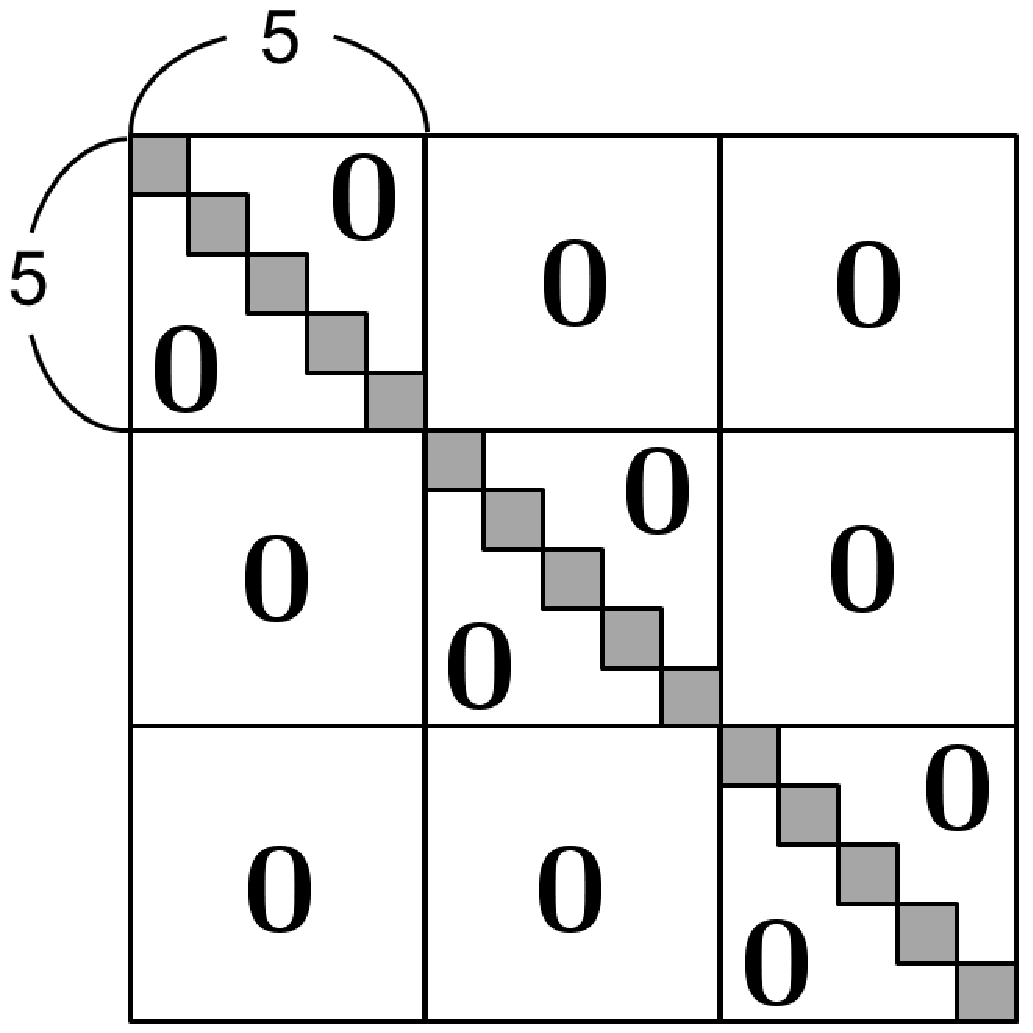
\includegraphics[width=0.8\hsize]{fig/GMM_1.pdf}
      \\ (a) diagonal \\(without -c1 and -c2 option)
     \end{center}
    \vspace{3mm}
    \begin{center}
     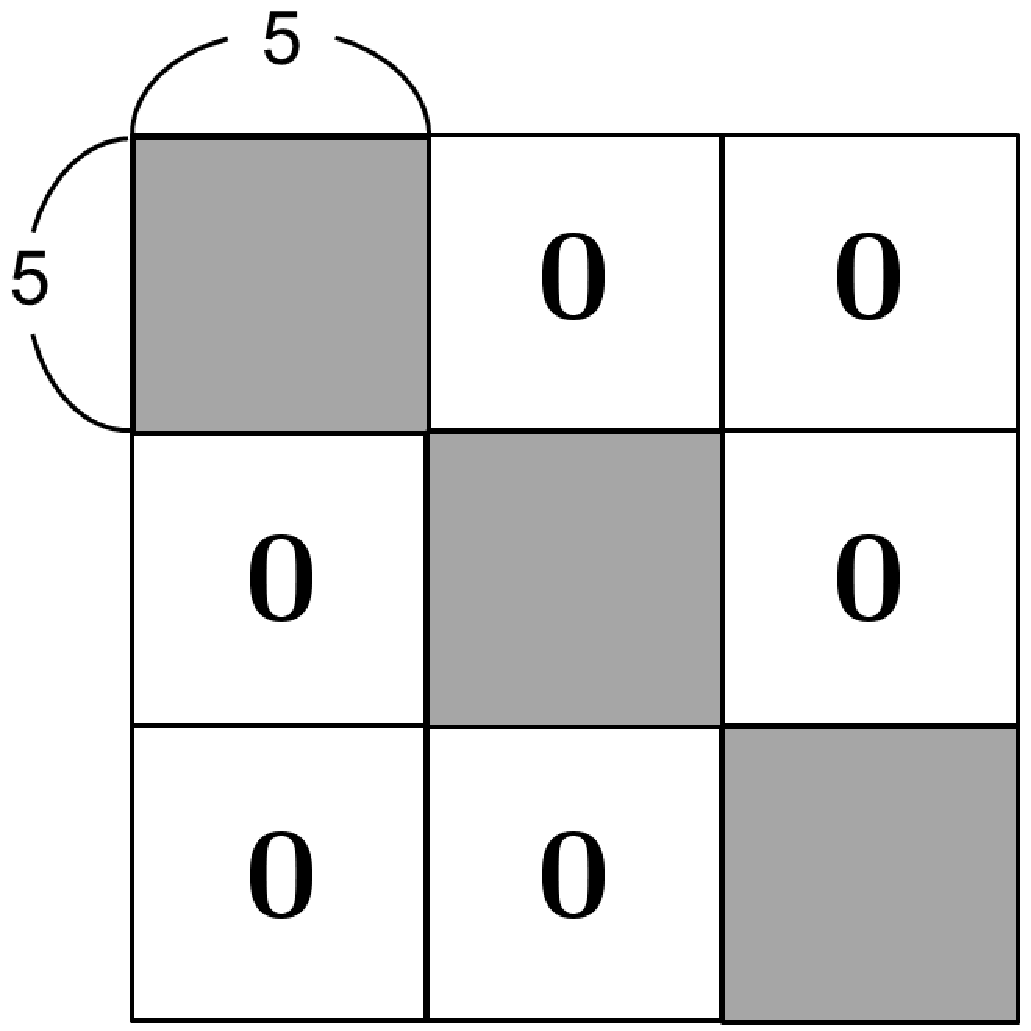
\includegraphics[width=0.8\hsize]{fig/GMM_3.pdf}
    \\ (c) block-wise full covariance \\(with -c2 option)
    \end{center}
   \end{minipage}
   \begin{minipage}[b]{0.45\hsize}
    \begin{center}
     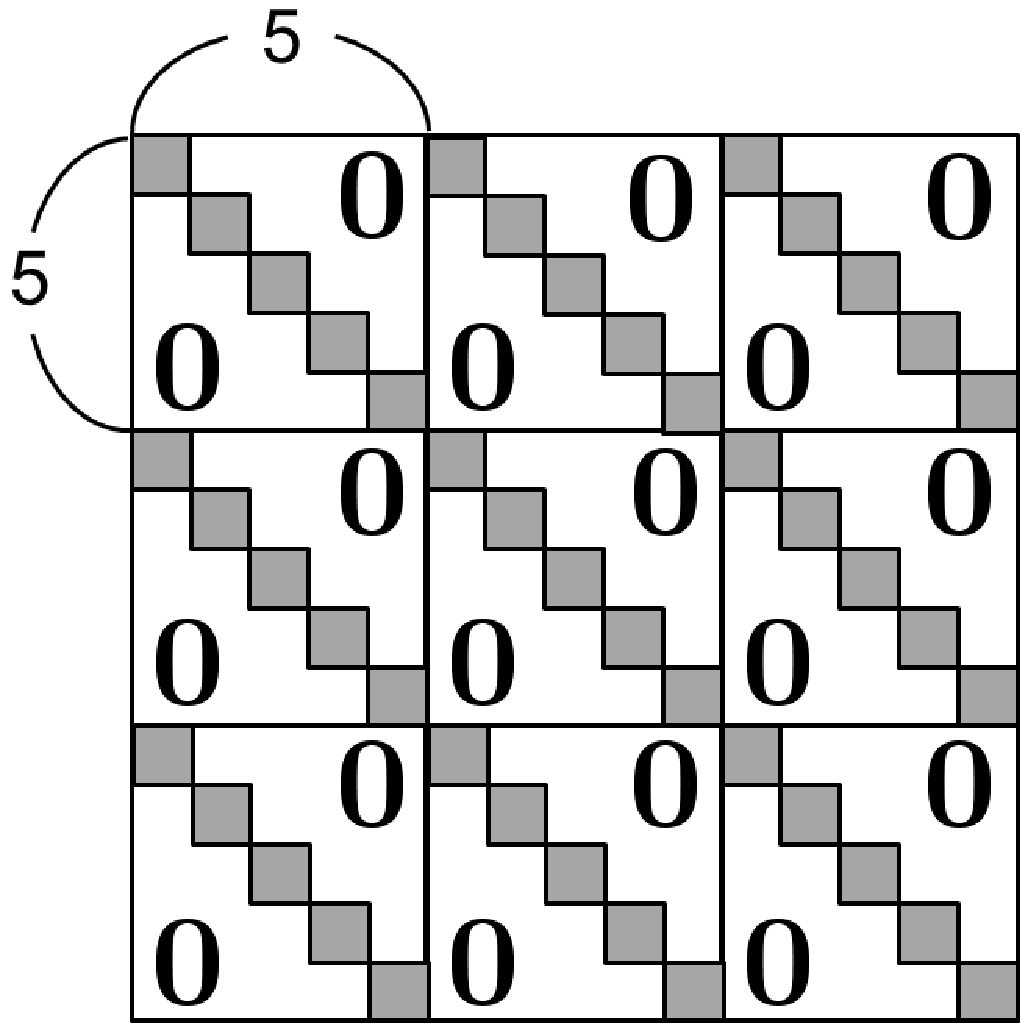
\includegraphics[width=0.8\hsize]{fig/GMM_2.pdf}
     \\ (b) inter-block correlation \\(with -c1 option)
    \end{center}
    \vspace{3mm}
    \begin{center}
     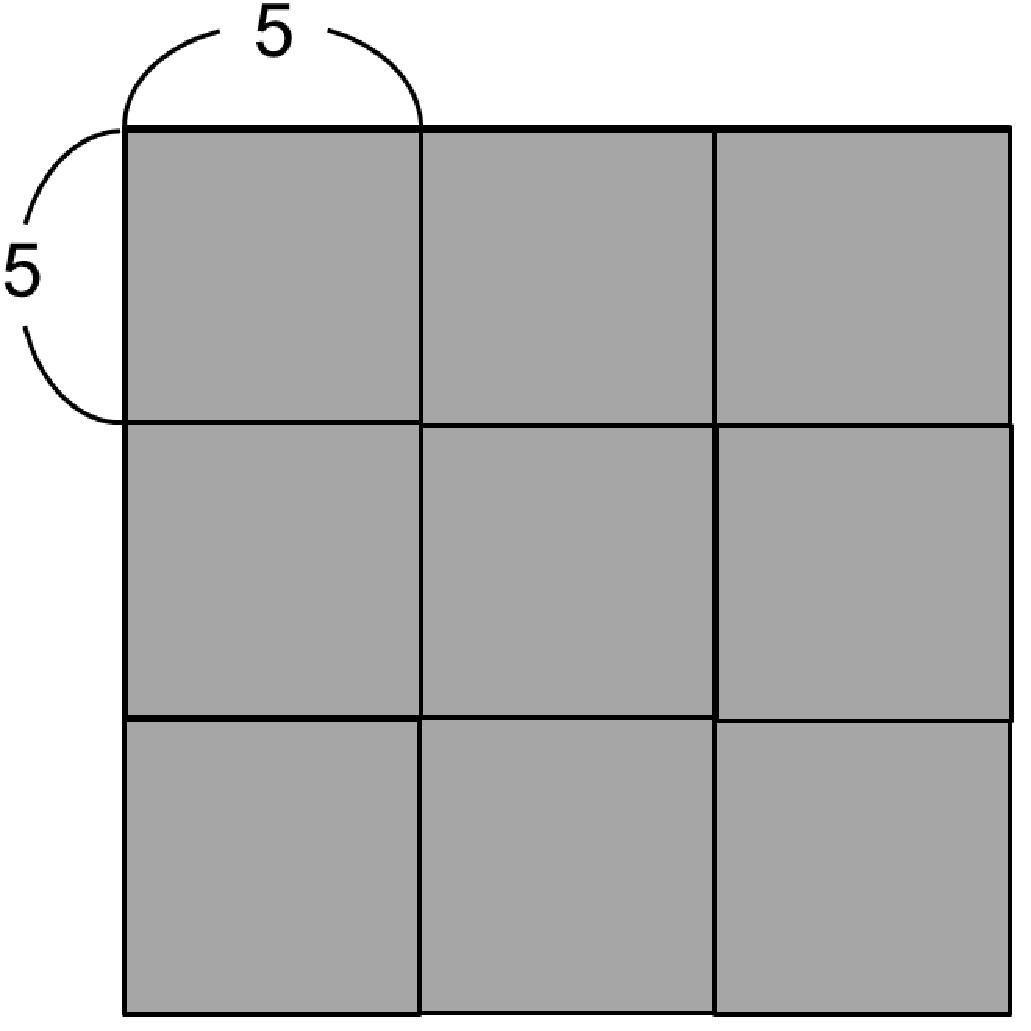
\includegraphics[width=0.8\hsize]{fig/GMM_4.pdf}
     \\ (d) full covariance \\(with both -c1 and -c2 option)
    \end{center}
   \end{minipage}
  \end{tabular}
 \end{center}
 \caption{Examples of the structure of covariance matrix}
 \label{fig:gmm_c1}
 \end{figure}
\end{qsection}

\newpage

\begin{qsection}{NOTICE}
\begin{itemize}
\item The -e option specifies a threshold for the change of average
 log-likelihood for training data at each iteration.
\item The -F option specifies a GMM initial parameter file in which
weight, mean, and variance parameters must be aligned in the same
order as output.
\item The -B option specifies the size of each blocks in covariance matrix.
\item The -c1 and -c2 option must be used with -B option. Without -c1 and
-c2 option, a diagonal covariance can be obtained.
\end{itemize}
\end{qsection}

\begin{qsection}{SEE ALSO}
\hyperlink{gmmp}{gmmp},
\hyperlink{lbg}{lbg}
\end{qsection}
